\documentclass[oneside,a4paper,titlepage]{article}
\usepackage{color}
\usepackage{hyperref}
\usepackage{graphicx}
\usepackage[utf8]{inputenc}

\title{Pumpkin basic Manual}

\author{Rafael de Paula Paiva,
		\texttt{08.paiva@gmail.com}
		}
		
%\thanks{Dr. Emiu Petriu,\\ 
%		M. Vinicius Prado,\\
%		M. Tiago Eustakio}
		
\date{\today}

\begin{document}

\maketitle
\tableofcontents
\newpage

\section{First steps}

\subsection{Environment}

The Pumpkin project is based on ROS (Robot Operatin System), a framework and system that creates a base layer for distributed systems.

The system is intended to be run into, at least, two different devices. One of them will hold the core system, that read from the sensors, and command the servos. The others devices will run the GUI (Graphical User Interface).

\subsubsection{Installing ROS}

The ROS, by default, runs on Linux, but there is possible to install ROS in other systems. The Pumpkin was developed and tested in the Ubuntu distro, so this is the recommended disto, although it can be used other distros. But the recomendation to Linux stills.

The installation guide can be found in: \href{http://wiki.ros.org/indigo/Installation}{ROS Indigo installation guide page}.

The Pumpkin was developed in the ROS Indigo, since it has more support. So, it's sugested that install this version. To be sure to have everything OK, try to install the desktop-full version.

\subsubsection{Necessary ROS packages}

There is others ROS packages after the basic installation that the Pumpkin system use. All the subsequent packages are debian-like installation packages. They can be installed running a installation program, like the \textit{synaptic}, or the \textit{Ubuntu Software Centre} programm, or running the command below in a terminal:

\begin{center}
\texttt{sudo apt-get install \textbf{<package-name>}}
\end{center}


All the packages below will contain the ROS distro name. For example, if you run the Indigo distro, the packages to be installed will be named: \texttt{ros-indigo-...}, but if you are running the Jade distro, the packages will be named: \texttt{ros-jade-...}.

For each package shown below, install it using one of each option. Using a installation program, or by command-line.

The first package to install is the \textbf{actionlib}, to run the Action Service. The name of the package is:

\begin{center}
\texttt{ros-<distro>-actionlib}
\end{center}

(override the <distro> by the distro used, as explained above).

After that, it is necessary to install the \textit{MoveIt!}. This package if for trajectory planning. To install it, install this package:

\begin{center}
\texttt{ros-<distro>-moveit-ros}
\end{center}

The next component is the Rosserial. It is necessary to communicate to the Arduino board. To install it, there is two packages to be installed:

\begin{center}
\texttt{ros-<distro>-rosserial-arduino}\\
	and\\
\texttt{ros-<distro>-rosserial-server}
\end{center}
 
\subsubsection{QT}

The ROS GUI is made in QT. This section is only necessary to do in the device to run the GUI, but it can also be done in the machine that run the Pumpkin core.

\textbf{Note: } It is recommended to install the QT in the machine that will run the pumpkin core, since it has some visual tools that will use, also, QT.

To run the GUI, install the package: 

\begin{center}
\texttt{libqt4-dev}.
\end{center}

\subsection{Pumpkin Installation}

First of all, it is necessary to download the Pumpkin project to the machines. Create a folder in the machine to the project be in.

...

\paragraph{Atention: } These instructions above is for all machine that will run the Pumpkin system.

\paragraph{Note: } All the commands shown below is to be ran in the same folder that the project was downloaded.

Now, it's time to build the system.

\subsubsection{Building the core packages}

This instructions below is for the machine that will run the Pumpkin core, that is, the machine that have direct control with the servos, and connections with the sensors.

In theory, this machine should be enbedded in the robot.

After downloading the project, run the command:

\begin{center}
\texttt{catkin\_make}
\end{center}

to build the project. Sometimes it is necessary to run the command again, if the first time some erros may have been shown.

If you don't want to install QT on the machine that will run the GUI, run this command to exclude the GUI package:

\begin{center}
\texttt{catkin\_make --pkg pumpkin\_messages pumpkin pumpkin\_interface}
\end{center}

\subsubsection{Building the GUI packages}

This steps is to build the GUI for the Pumpkin.

If both the machine are the same, and it was run \texttt{catkin\_make} in the step before, nothing more have to be done. So, just run the command.

Otherwise, if the machine are not the same, there is two options:

The first option, run \texttt{catkin\_make} to build everything. But this is not necessary.

The second option is just to build the GUI. To do it, run:

\begin{center}
\texttt{catkin\_make --pkg pumpkin\_messages pumpkin\_qt}
\end{center}

\subsection{Last environment settings}

For now, the both systems may run, but we need to configure the network environment to both be able to communicate.

The first thing to do is to be sure that both machines are on the same local network, i. e. they are on the same WiFi network.

\subsection{Running Pumpkin}


\section{Using Pumpkin}

\subsection{Basics}

Pumpkin is a robot made, until now, to play recorded movements, and to be able to concatenate movements.

Here are some terms that will be used in this project:

\begin{description}
	\item[Movement] A sequence of positions of the robot parts over time, that, combined, form a movement, as a normal movement as you can imagine. Examples are: shaking hand, doing a ``bye'', etc.
	
	\item[Playback file] Is a full movement that is recorded into a file, to be played later. The file contains the value of the sensors of the robot over the time since the start of the movement.
	
	\item[Playback] This is the action of the robot executing the movement saved in a \emph{playback file}.
	
	\item[Record] Is the action of create a \emph{playback file}, saving, over a period of time, the value of sensors. The movement is done moving the robot parts, like a ragdoll.
	
	\item[Planning] Is a computational process that create a temporary movement to be executed between two defined positions passed as the entry of this process.
	
	\item[Scene] Is a sequence of \emph{playback files} that are executed in order, composing a new movement. Between each pair of movement, the Pumpkin \emph{plans} the xxx, as the overall movement appears more natural. This new movement, although, is not saved as a new movement, since this new movement depends only of the sequence of \emph{playback files}, repeating this sequence recreates this \emph{scene}
\end{description}

\paragraph{Note: } For security reasons, all the motors starts turned off, and also they will be turned off after finishing a \emph{playback} or \emph{scene}. Obviously, the motors have to be turned off to be able to record a scene.

To command the robot, a prior, use the GUI, since it covers all the functionalities of the robot, and also is made to be ease to use.

\subsection{The PumpkinQT}

Now, for the basic usage of the Pumpkin system. The GUI was designed to help for the basic usage of the robot.

The first window that you may see is the configuration window. This window run only once as the core system still runs in the main machine, it may appear if the core system restarts.

\begin{figure}[h!]
	\centering
	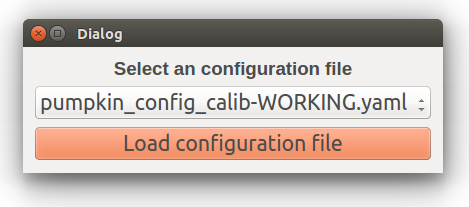
\includegraphics[width=0.8\textwidth]{load_config}
	\caption{Load Config dialog}
	\label{fig:load_config}
\end{figure}

The only thing to do here is select a configuration file from the list, and press the button.

As said, this dialog only show once. So, after selecting the configuration file, you go to the main window. If you have ran the configuration before, the main window will be shown directly.

\begin{figure}[h!]
	\centering
	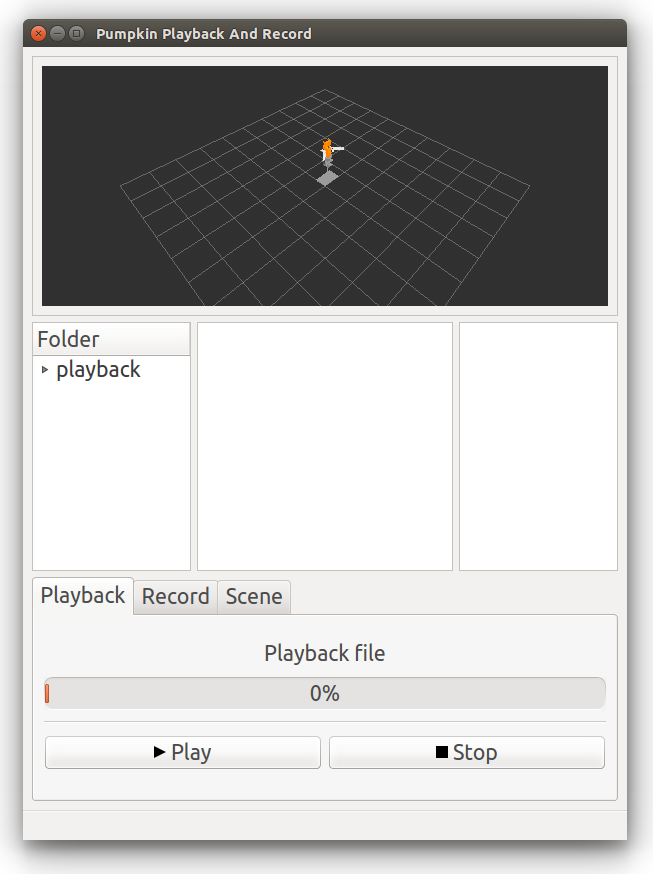
\includegraphics[width=0.8\textwidth]{main_window}
	\caption[Main Window]{the PumpkinQT main window, an ease way to use the Pumpkin}
	\label{fig:main_window}
\end{figure}

At a first glance, there is, in the topmost part, a 3D model of the robot, to have a view of the Pumpkin.

Under this view, there are thre lists:

\begin{itemize}
	\item The left one is to show the folder tree to view the folders that holds the recorded playback files, in a tree model (that is, the children folders are indented from the parent folder).

	\item The center one is to show the list of playback files that are inside the selected folder. This list start empty since no folder is selected. As you select a folder, the list of files are shown, for the current folder.
	
	\item The right one is the list of selected playback files to play a scene. The scene is covered after.
\end{itemize}

And the bottom part of the window are the actions controls. They're displayed in different tabs, each one representing a different functions.

\subsubsection{Playback}
\label{subsec:playback}
	This function is to order the robot to execute a previous recorded playback. To do this, first, an playback file must be selected. As it's selected, the name of the file will be displayed where initially is written \textbf{Playback file}.
	
	\begin{figure}[h]
		\centering
		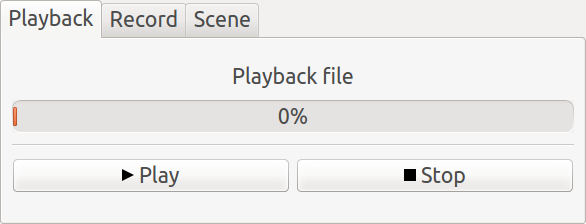
\includegraphics[width=0.8\textwidth]{playback_tab}
		\caption[Playback Tab]{The playback tab is to execute one movement}
		\label{fig:playback_tab}
	\end{figure}
	
	To playback, just press the \emph{Play} button (as seen in: \ref{fig:playback_tab}). As you press this button, you will see the progress bar starting filling up. This is because this progress bar show the completed percentage of the movement. You will see, also, that the \emph{Play} button will not be more clickable, and this is logically because you are in the middle of a movement.
	
	While the robot is executing the movement, you can press the stop button, to stop the execution of the movement. Obviously, the button will only be clicable when the robot is executing a movement.
	
\subsubsection{Record}
\label{subsec:record}
	This function is to record a new movement. To this, you have, first, to select a folder. You can, also, select a file in the playback file list to override a playback file.
	
	\begin{figure}[h]
		\centering
		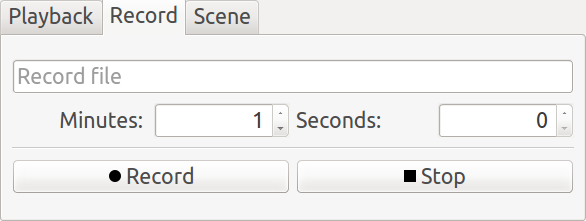
\includegraphics[width=0.8\textwidth]{record_tab}
		\caption[Record Tab]{The record tab is to record new movements}
		\label{fig:record_tab}
	\end{figure}
	
	The first thing to do here is to write the \emph{playback file} name (in the entry, that maybe show a light gray ``Record file'' text.). You can, also, overrite a movement, selecting a file, and the \emph{playback file} name will be in the entry. Note that writing an existing \emph{playback file} (in the same folder) will also overrite that file.
	
	After that, a time limit for the movement is needed to be set (in the tho slots, one for the minutes value, and other for the seconds value). The recording will stop when the time limit reachs, or the \emph{Stop} button is pressed in the middle of a recording.
	
	As the record starts, you will see that the entries for the time limit will not be able to modify, but the values in there will start changing. This is because these entries will show the elapsed time since the begining of the recording.
	
\subsubsection{Scene}
\label{subsec:scene}
	This is, for now, is the most advance function of the robot. This is the only function that will use the right list (in the middle part of the \ref{fig:main_window}).

	\begin{figure}[h]
		\centering
		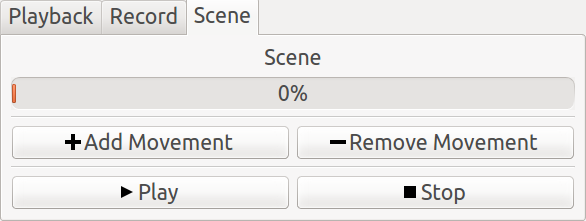
\includegraphics[width=0.8\textwidth]{scene_tab}
		\caption[Scene Tab]{The scene tab is to play a sequence of movements}
		\label{fig:scene_tab}
	\end{figure}
	
	The first thing to do is to create the \emph{playback file} list. To do that, the two buttons in the upper part of the \emph{scene tab}.
	
	To add a movement to the \emph{scene}, select a playback file (as for \emph{playback} this file), and then click the \emph{Add movement} button.
	
	To remove a movement from the scene, select a file from the scene list, and click the \emph{Remove movement} button.
	
	And to change the order of the movement, just ``drag and drop'' the \emph{playback file} from the \emph{scene list} and put it in the desired position.
	
	After that, play the scene clicking the \emph{Play} button. This is like a playback, but all the movements are executed in order they appear in the \emph{scene list}. Remember that, as the playback, you can stop at any moment.
	
	The progress bar and the text that you see is to indicate the overall completion of the scene. The progress bar is equal to the playback, indicate the completed percentage of the movement, or the planning, and the text indicate each movement (or planning between movements) is being executed in that moment.
	
\subsection{Other PumpkinQT ...}

There are other two ... that the PumpkinQT is able to do. They're accessed by the menu of the \emph{Main Window} (\ref{fig:main_window}). 

\subsubsection{Manage files and folders}

\begin{figure}[h]
	\centering
	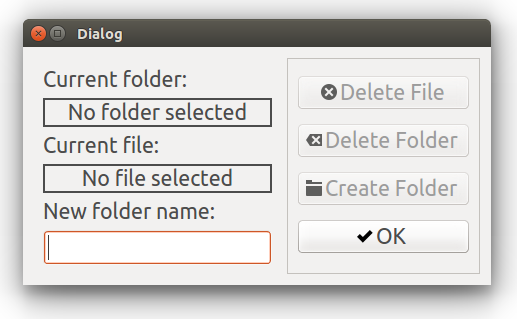
\includegraphics[width=0.8\textwidth]{manage_files}
	\caption[Files Manager]{The files manager dialog is to manage the files and folders of playback}
	\label{fig:manage_files}
\end{figure}

The \emph{Files manager dialog} (Figure \ref{fig:manage_files}) is used to manage the files and folders. To organize the \emph{playback files} better, they're disposed in different folders. So, you are able to create, and delete these folders. And also delete any movement file thay you doesn't want anymore.

{\color{red}
\paragraph{ATENTION!} As this system runs in a network environment, all these actions are request to the OS that runs the core of the Pumpkin. So, it is not possible to recover a deleted movement, or folder.
}

If you open the dialog without selecting any folder, you will see it as shown in the figure \ref{fig:manage_files}. But, as soon you select a folder, in the space you see ``No folder selected'', you will see the name of the selected folder. In the same way, as soon you select a file, you see the name of the selected file (in this case, with the full path), where is shown ``No file selected''.

The entry, in the botton left part of the dialog, is where you write the name of a new folder, in case you want to create one.

To do any job, just click on the respect button in the right part of the dialog window:

\begin{description}
	\item[Delete File] Delete the selected file. This button will not be clickable until you select a file.
	
	\item[Delete Folder] Delete the selected folder. This button will not be clickable until you select a folder.
	
	\item[Create Folder] Create a new folder under the selected folder (as a child folder). First, you have to select a folder to do that.
\end{description}

To close the dialog, just click the \emph{OK} button.

\paragraph{Note: } Creating a new playback file is done in the \emph{Record} (Section \ref{subsec:record}).

\subsubsection{SSC Move Command Sender}

The other resource is more advanced, and was created to debugging purpose. You can test it too, but is \textbf{\color{red} HIGHLY NOT RECOMMENDED} in case you are not developing for Pumpkin.

\begin{figure}[h]
	\centering
	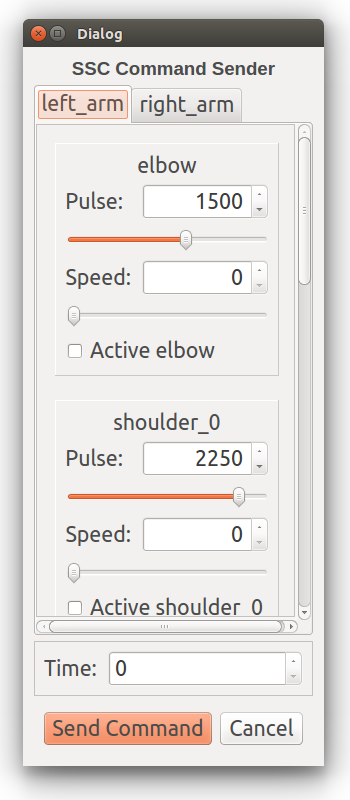
\includegraphics[width=0.8\textwidth]{ssc}
	\caption[SSC Move Command Sender]{The SSC Move Command Sender is a more advanced resource, to send commands directly to the servos}
	\label{fig:ssc}
\end{figure}

First of all, if you don't know what is a Servo, it probably is not for you. Just don't touch in this window. Press the \emph{Cancel} button and close it.

This is a raw command sender to the robot servos. As, until now, the robot use an SSC to send command to this joints, this dialog is used to that: send commands to the joint.

The command dialog is divided into tabs, each tab contains a robot part (this is just to organize better the joint panel). Each pannel inside a tab is designed for one joint.

The first thing to notice, for each panel, is there is a check box. Leave it checked to send the specific command to the servo related to that joint, but if you want to leave that servo out of the command, uncheck it. After that, just set the value for the pulse width. If you wish to set a speed to the servo, just set the speed value over $0$ (zero).

The last thing before sending the command is the time value (the time limit to each servo have to be). If you want to send the time among the info, just set the value above $0$ (zero).

Click the \emph{Send Command} button to send the button. You can send any ammount of commands you wish. After that, click on the \emph{Cancel} button to close the dialog.

\section{Understanding the project}

\end{document}
